% !TEX root = ../../Beamer/09ComplexFrames/09ComplexFrames.tex


\begin{tikzpicture}[scale=\scale]


	\small
	\coordinate (A) at (0,0);
	\coordinate (AB) at (0,3);
	\coordinate (B) at (4,3);
	\coordinate (BC) at (8,3);
	\coordinate (C) at (8,5);
	\coordinate (G) at (2.75,4.25);
	\coordinate (F) at (1.425,0.5);
	\coordinate (R) at (5.78,0.5);
	\coordinate (P) at (10.5,1.5);


	\gettikzxy{(A)}{\Ax}{\Ay}
	\gettikzxy{(AB)}{\ABx}{\ABy}
	\gettikzxy{(B)}{\Bx}{\By}
	\gettikzxy{(BC)}{\BCx}{\BCy}
	\gettikzxy{(C)}{\Cx}{\Cy}
	\gettikzxy{(G)}{\Gx}{\Gy}
	\gettikzxy{(F)}{\Fx}{\Fy}
	\gettikzxy{(R)}{\Rx}{\Ry}
	\gettikzxy{(P)}{\Px}{\Py}

	\def\hi{0.25}

	% \coordinate (B) at (-0.55,-0.25) node {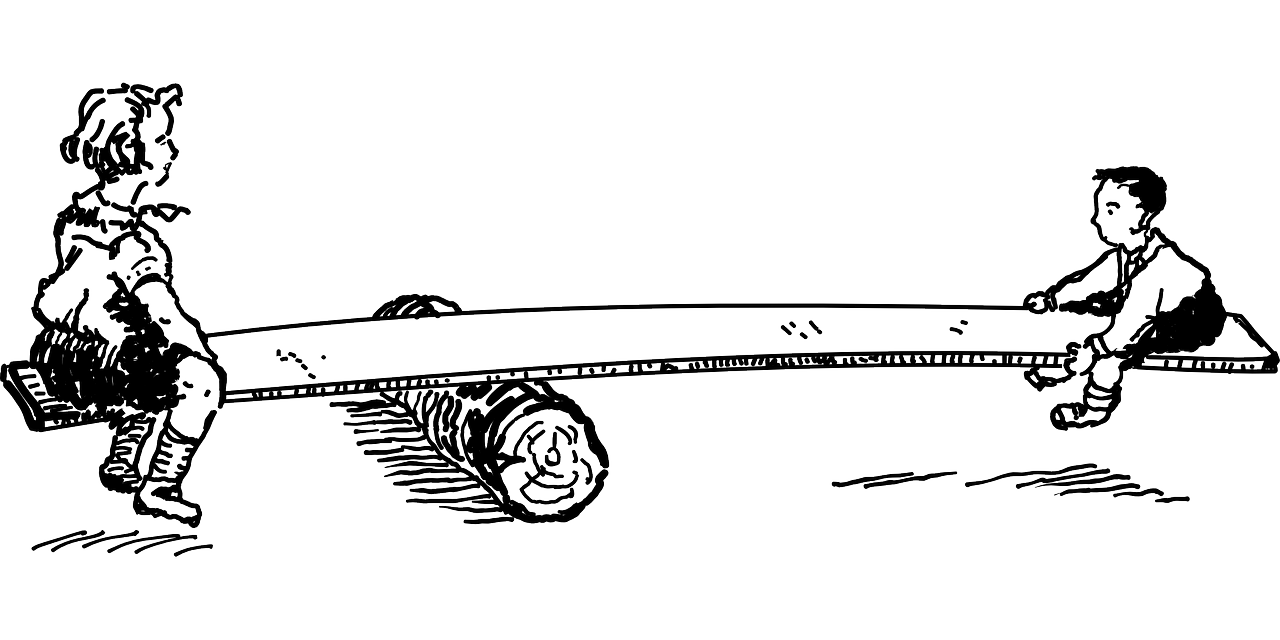
\includegraphics[scale=0.15]{../../images/teeter-totter.png}};
	\node[yshift=0.75cm,xshift=-0.125cm] at (B) {\includegraphics[scale=0.465]{../../figs/09CF/orangeSportsCar.png}};

	\filldraw[fill=LightGoldenrod3] (\Ax-\hi cm, \Ay)arc(180:360:\hi)--(\Ax+\hi cm, \By-\hi cm)--(\Bx-\hi cm,\By-\hi cm)arc(-90:90:\hi)--(\Ax-\hi cm,\By+\hi cm)--cycle;
	\filldraw[fill=LightGoldenrod3] (\Cx-\hi cm, \Cy)arc(180:0:\hi)--(\Cx+\hi cm,\By-\hi cm)--(\Bx+\hi cm, \By-\hi cm)arc(270:90:\hi)--(\Cx-\hi cm,\By+\hi cm)--cycle;

	\shade[right color=DarkOliveGreen2, left color=DarkOliveGreen4] ($(C)+(0.75,1.5)$)rectangle($(C)+(1.5,-3)$);
	\shade[bottom color=DarkOliveGreen2, top color=DarkOliveGreen4] ($(A)+(-1.5,-0.75)$)rectangle($(A)+(1.5,-1.75)$);
	\shadedraw[ball color=DarkOliveGreen3] (B) circle (5pt);
	\fill (G) circle (2pt)node[xshift=-0.25cm]{$G$};
	\PinnedConnection{A}{DarkOliveGreen3}{black}{0.75}{0.1}
	\PinnedConnection[90]{C}{DarkOliveGreen3}{black}{0.75}{0.1}
	\node[yshift=-0.25cm] at (B) {$B$};
	\node[xshift=-0.375cm] at (A) {$A$};
	\node[yshift=0.375cm] at (C) {$C$};

	\draw (\Ax, \ABy-2*\hi cm) -- +(0,-2);
	\draw (\Gx, \ABy-2*\hi cm) -- +(0,-2);
	\draw (\Bx, \ABy-4*\hi cm) -- +(0,-1.5);
	\draw (\Cx, \ABy-2*\hi cm) -- +(0,-2);
	\draw (\Fx, \ABy-2*\hi cm) -- +(0,-2);
	\draw (\Rx, \ABy-2*\hi cm) -- +(0,-2);
	\draw (\Cx+1cm, \Cy) -- (\Px+3*\hi cm,\Cy);
	\draw (\Bx+0.5cm, \By) -- (\Px+3*\hi cm,\By);
	\draw (\Ax+0.5cm, \Ay) -- (\Px+3*\hi cm,\Ay);

	\footnotesize
	\draw[latex-latex] (\Ax,\Py)--node[fill=white,inner sep=0.5mm,rotate=90]{$710\,$mm}(\Fx,\Py);
	\draw[latex-latex] (\Fx,\Py)--node[fill=white,inner sep=0.5mm,rotate=90]{$660\,$mm}(\Gx,\Py);
	\draw[latex-latex] (\Gx,\Py)--node[fill=white,inner sep=0.5mm,rotate=90]{$610\,$mm}(\Bx,\Py);
	\draw[latex-latex] (\Bx,\Py)--node[fill=white,inner sep=0.5mm,rotate=90]{$890\,$mm}(\Rx,\Py);
	\draw[latex-latex] (\Rx,\Py)--node[fill=white,inner sep=0.5mm,rotate=90]{$1110\,$mm}(\Cx,\Py);
	\draw[latex-latex] (\Px,\Cy)--node[fill=white,inner sep=0.5mm]{$1050\,$mm}(\Px,\By);
	\draw[latex-latex] (\Px,\By)--node[fill=white,inner sep=0.5mm]{$1525\,$mm}(\Px,\Ay);


\end{tikzpicture}
